\documentclass[journal,twocolumn]{IEEEtran}
\usepackage{slashbox,graphicx,times,amsmath,amssymb,cite,subfigure,stfloats,booktabs, url,multirow,afterpage}
\usepackage[lined,ruled]{algorithm2e}
\allowdisplaybreaks

\makeatletter
\newcommand{\rmnum}[1]{\romannumeral #1}
\newcommand{\Rmnum}[1]{\expandafter\@slowromancap\romannumeral #1@}
\makeatother


\begin{document}
\title{Patch Learning}

\author{Dongrui~Wu,~\IEEEmembership{Fellow,~IEEE} and Jerry M. Mendel,~\IEEEmembership{Life Fellow, IEEE}
\thanks{D.~Wu is with the Key Laboratory of Image Processing and Intelligent Control (Huazhong University of Science and Technology), Ministry of Education, China. He is also with the School of Artificial Intelligence and Automation, Huazhong University of Science and Technology, Wuhan, China. Email: drwu@hust.edu.cn.}
\thanks{J.M. Mendel is with the Ming Hsieh Department of Electrical Engineering, University of Southern California, Los Angeles, CA, USA. He is also with the College of Artificial Intelligence, Tianjin Normal University, Tianjin, China. Email: mendel@sipi.usc.edu.}}

\markboth{IEEE Transactions on Fuzzy Systems, 2023}%
{Shell \MakeLowercase{\textit{et al.}}: Bare Demo of IEEEtran.cls for IEEE Journals}
\maketitle

\begin{abstract}
There have been different strategies to improve the performance of a machine learning model, e.g., increasing the depth, width, and/or nonlinearity of the model, and using ensemble learning to aggregate multiple base/weak learners in parallel or in series. This paper proposes a novel strategy called patch learning (PL) for this problem. It consists of three steps: 1) train an initial global model using all training data; 2) identify  from the initial global model the patches which contribute the most to the learning error, and train a (local) patch model for each such patch; and, 3) update the global model using training data that do not fall into any patch. To use a PL model, we first determine if the input falls into any patch. If yes, then the corresponding patch model is used to compute the output. Otherwise, the global model is used. We explain in detail how PL can be implemented using fuzzy systems. Five regression problems on 1D/2D/3D curve fitting, nonlinear system identification, and chaotic time-series prediction, verified its effectiveness. To our knowledge, the PL idea has not appeared in the literature before, and it opens up a promising new line of research in machine learning.
\end{abstract}

\begin{IEEEkeywords}
Ensemble learning, fuzzy system, patch learning, regression
\end{IEEEkeywords}

\IEEEpeerreviewmaketitle

\section{Introduction}

Machine learning has been widely used in our everyday life, e.g., face recognition \cite{Zhao2003}, natural language processing \cite{Collobert2011}, recommender systems \cite{Wang2015b}, affective computing \cite{drwuVRST2010,drwuMTALR2021}, brain-computer interfaces \cite{drwuiGS2019,drwuEA2020}, etc. However, training a high-performance machine learning model is usually a challenging and iterative process, relying on experience and trial-and-error: a simple model is first designed; if its performance is not satisfactory, then some remedies are taken to enhance it.

There have been different strategies to enhance the performance of an under-performing machine learning model:
\begin{enumerate}
\item \emph{Use a single deeper model}. For example, when the performance of a simple multi-layer perceptron neural network \cite{Bishop1995} is not satisfactory, a deep learning model \cite{LeCun2015,He2016}, which has tens or even hundreds of layers, can then be trained. When the performance of a conventional fuzzy system is not enough, a hierarchical fuzzy system \cite{Raju1991} with multiple layers can then be designed.

\item \emph{Use a single broader (wider) model}. For example, when the performance of a simple multi-layer perceptron neural network is not enough, more nodes can be added to each hidden layer \cite{Bishop1995}, or enhancement nodes can be added to convert it into a broad learning system \cite{Chen2018b}. When the performance of a simple fuzzy system is not enough, more membership functions (MFs) or rules can be added to make it wider \cite{Mendel2017}; or, in other words, to sculpt the state space more finely \cite{Mendel2018}.

\item \emph{Use a single more non-linear model}. For example, when the performance of a simple linear regression model is not enough, a non-linear regression model like support vector regression using the radial basis function kernel \cite{Smola2004} can be used. When the performance of a simple fuzzy system with constant rule consequents are not enough, a more non-linear Takagi-Sugeno-Kang (TSK) fuzzy system \cite{Takagi1985}, whose rule consequents are linear or non-linear functions of the inputs, can be considered. When the performance of a type-1 fuzzy system is not enough, a more non-linear interval type-2 fuzzy system \cite{drwuEAAI2006,drwuISA2006} can be considered. Note that generally a deeper (broader) model has more non-linearity than a shallower (narrower) model. So, the previous two strategies are also implicitly included in this one.

\item \emph{Connect multiple simple models (usually called base learners) in parallel}. This is a classic idea in ensemble learning \cite{Zhou2012}. For example, when the performance of a base learner is not enough, multiple base learners can be generated in parallel from different partitions of the training data (e.g., bootstrap \cite{Efron1993}, or cross-validation), from different combinations of features (e.g., random forests \cite{Breiman2001}), and/or using different machine learning approaches (e.g., neural networks, fuzzy systems, decision trees, etc.). These base learners can then be aggregated using majority voting (for classification) or averaging (for regression) for better and more robust performance. An illustration of the parallel ensemble learning approach is shown in Fig.~\ref{fig:Parallel}.

\item \emph{Connect multiple simple models (usually called weak learners) in series}. This is another classic idea in ensemble learning. For example, when the performance of a weak learner is not enough, multiple weak learners can be generated in series, each focusing on the hard examples that previous weak learners cannot learn correctly [e.g., AdaBoost \cite{Freund1997a}, illustrated in Fig.~\ref{fig:Serial}], or directly compensating the training error made by previous weak learners (e.g., gradient boosting machine \cite{Friedman2001}).
\end{enumerate}

\begin{figure}[htbp]\centering
\subfigure[]{\label{fig:Parallel}   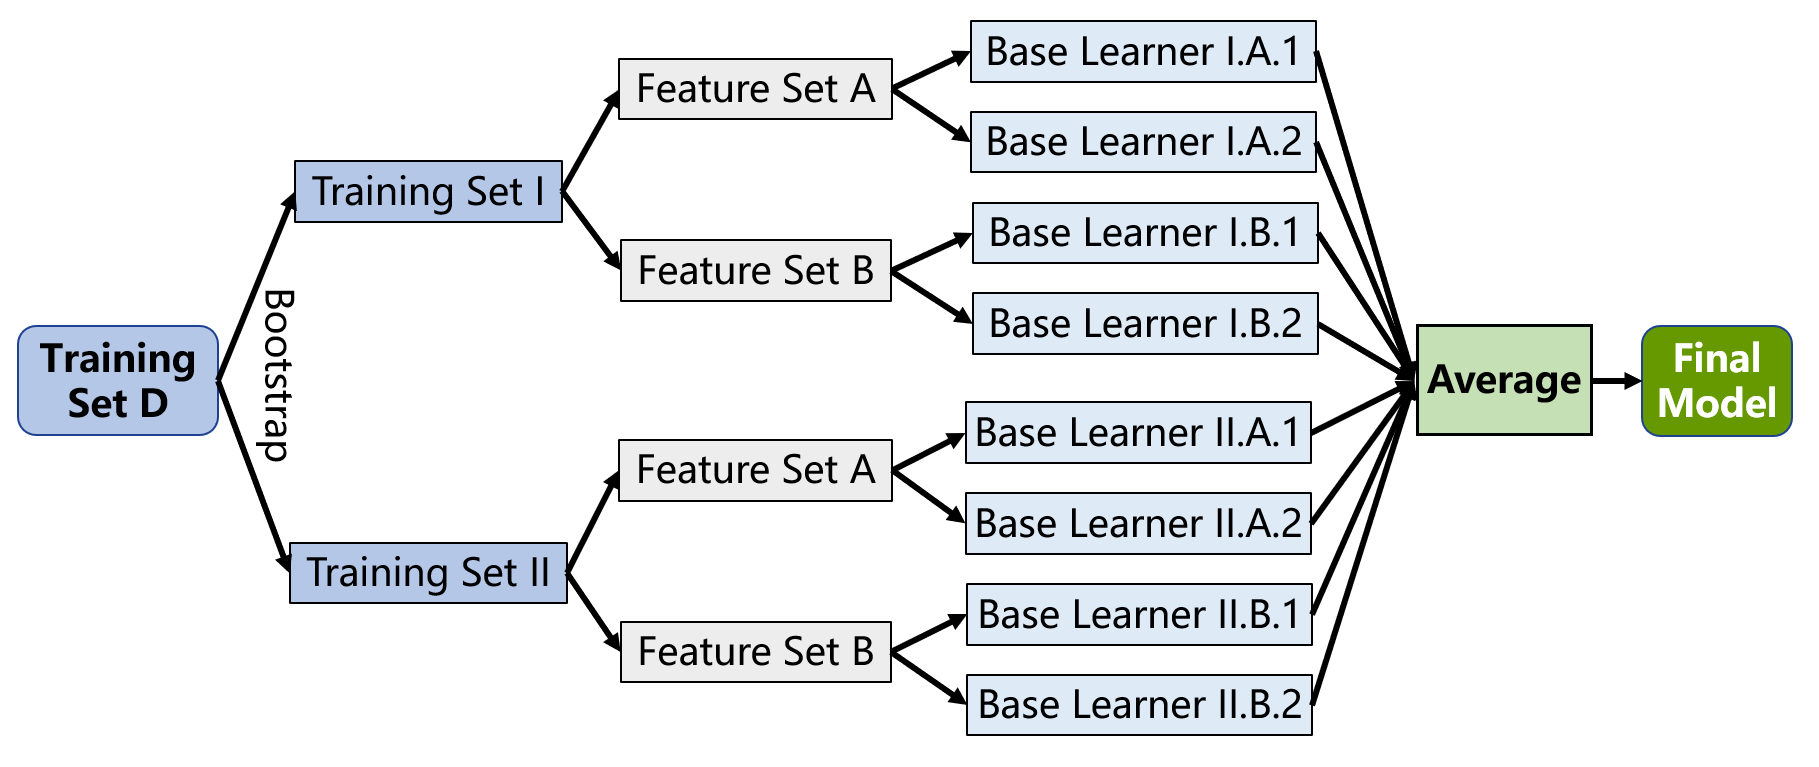
\includegraphics[width=\linewidth,clip]{Fig1a}}
\subfigure[]{\label{fig:Serial}    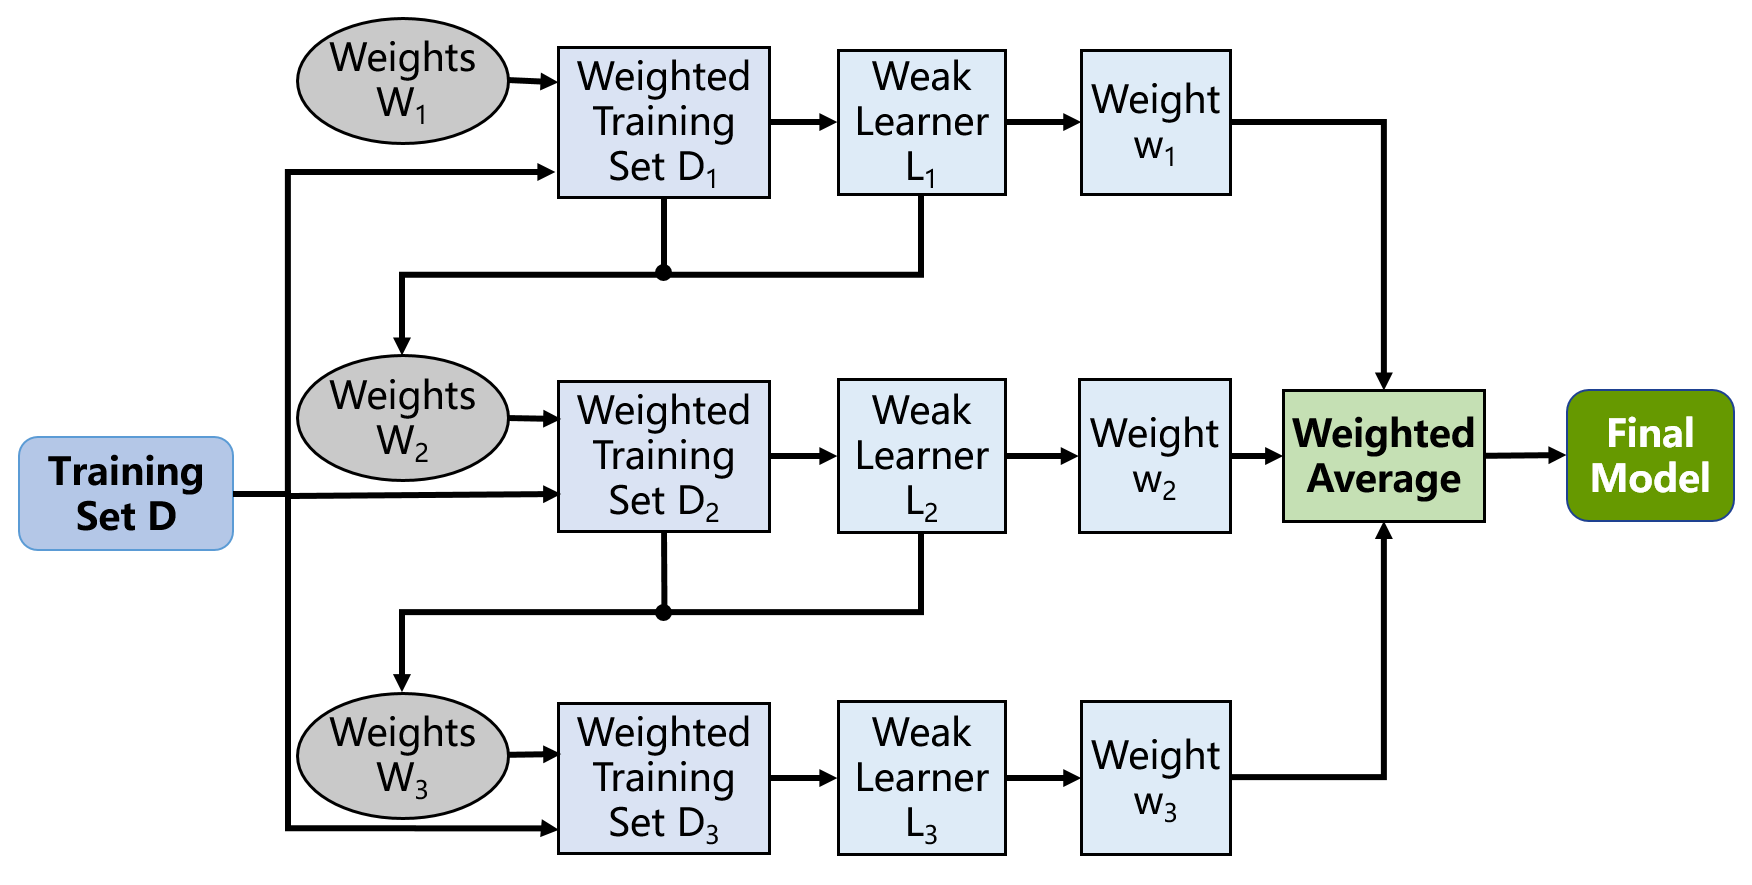
\includegraphics[width=\linewidth,clip]{Fig1b}}
\subfigure[]{\label{fig:Patch}    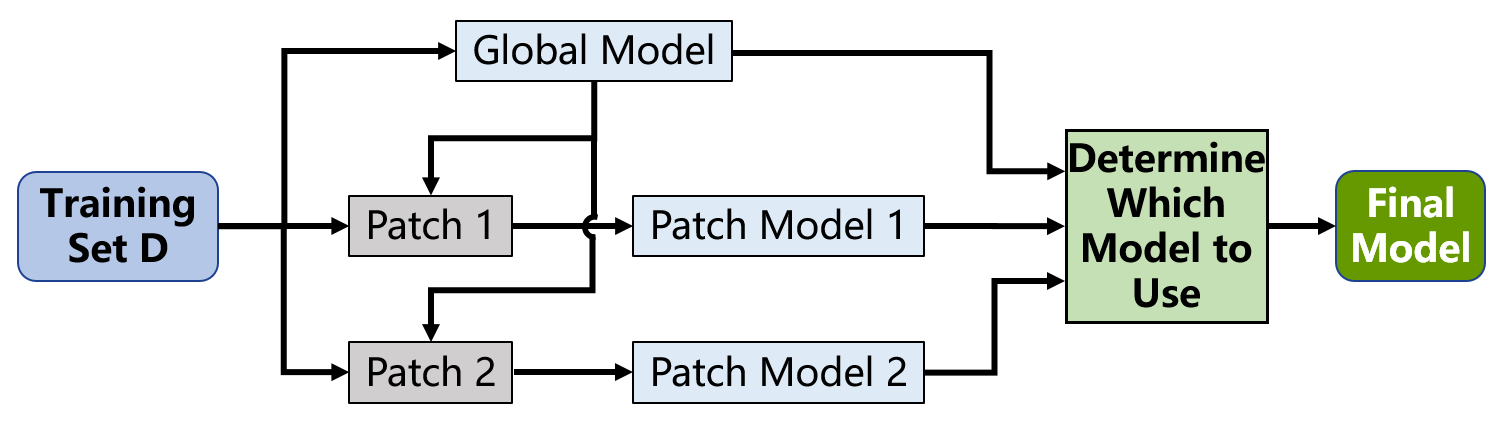
\includegraphics[width=.8\linewidth,clip]{Fig1c}}
\caption{Strategies for connecting multiple simple models for better performance. (a) parallel ensemble learning; (b) serial ensemble learning (AdaBoost \cite{Freund1997a}); and, (c) PL.} \label{fig:EL}
\end{figure}

This paper proposes \emph{patch learning} (PL), which connects multiple simple models both in parallel and in series to improve the learning performance, as illustrated in Fig.~\ref{fig:Patch}. It first trains a global model using all training data, identifies the input regions that give rise to large learning errors, and then designs a patch model for each such region to reduce the overall learning error. The patch models are parallel to and independent of each other, but they are all generated based on the initial global model (and hence in series to the global model). To our knowledge, this idea has not been explored before. We demonstrate the feasibility of PL using fuzzy systems in five regression problems.

The remainder of this paper is organized as follows: Section~\ref{sect:PL} introduces the general idea of PL, and illustrates it by a simple regression problem. Section~\ref{sect:PLFS} describes in detail how PL can be implemented by fuzzy systems. Section~\ref{sect:experiments} presents five experiments on PL using fuzzy systems to demonstrate its feasibility. Section~\ref{sect:limitations} points out some limitations of the current PL approach, and hence opportunities for future research. Finally, Section~\ref{sect:conclusion} draws conclusions.

\section{PL: The General Idea} \label{sect:PL}

This section introduces the general idea of PL, and illustrates it by a simple example.

Formally, we define a \emph{patch} as a connected polyhedron in the input domain. For example, a patch in a 1D input domain is an interval, as shown in Fig.~\ref{fig:1Dpatch}, and a patch in a 2D input domain can be a rectangle, an ellipse, etc., as shown in Fig.~\ref{fig:2Dpatch}. For ease of implementation, in this paper we only consider polyhedra whose number of surfaces (sides) equals the dimensionality of the input domain, and each surface (side) is perpendicular to an axis of the input domain, e.g., an interval in the 1D input domain [Patches~1-3 in Fig.~\ref{fig:1Dpatch}], and a rectangle in the 2D input domain [each side is perpendicular to an axis, such as Patch~1 in Fig.~\ref{fig:2Dpatch}].

\begin{figure}[htbp]\centering
\subfigure[]{\label{fig:1Dpatch}   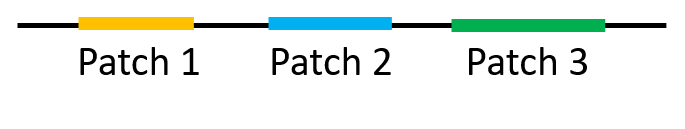
\includegraphics[width=.47\linewidth,clip]{Fig2a}}
\subfigure[]{\label{fig:2Dpatch}    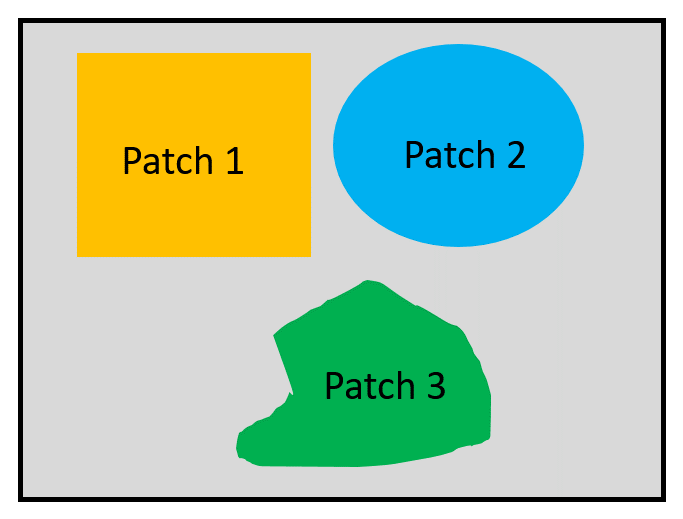
\includegraphics[width=.47\linewidth,clip]{Fig2b}}
\caption{Patches in 1D and 2D input domains.} \label{fig:patchs}
\end{figure}


\subsection{Steps of PL}

Given $L$, the number of patch models to be trained, PL consists of the following three steps:
\begin{enumerate}
\item Train an initial global model using all training data.
\item Identify $L$ patches from the initial global model, which contribute the most to the learning error, and train a (local) patch model for each such patch.
\item Update the global model using training data that do not fall into any patch.
\end{enumerate}
The rationale for the last step is that, when the default global model is first trained, it is forced to fit all training examples, some of which, e.g., those within the $L$ patches identified in Step (2), may be really difficult to fit. Since these difficult training examples have been handled by the patch models in Step (2), we can update the default global model to fit only the examples outside of the $L$ patches. This should be much easier than fitting all examples together, and hence the root mean squared error (RMSE) of the default global model may be reduced. Since in Step (3) the training examples for the updated global model are all outside of the patches, the updated global model is not suitable for inputs within any of the $L$ patches: although it can output an arbitrary value for such an input, this does not matter, since the patch models are used to handle such cases.

The idea of PL may be intuitively understood by making the following analogy. Consider a sculptor who is sculpting a human figure. After his first pass at this, the sculptor examines the entire figure and notices that improvements need to be made to certain parts of the figure. The sculptor does not throw out the entire figure and begin a new. Instead, he zooms into those parts that need more work, after which he blends in the refined portions of the figure with the rest of the figure. He continues such iterative refinements until he is satisfied with the entire figure. Each patch in PL is analogous to a part in the figure that needs more work. In traditional ensemble learning approaches, usually each base/weak learner also focuses on the entire figure, instead of a part of it.

\subsection{Determine the Optimal Number of Patch Models}

An important question in PL is how to determine $L$, the optimal number of patch models. Increasing $L$ is equivalent to increasing the model complexity in traditional machine learning. So, some analogy also applies here: generally, the training performance increases with $L$, but the test (generalization) performance may first increase and then decrease (indicating overfitting). Inspired from some common practices in traditional machine learning for reducing overfitting \cite{Duda2000,Hastie2009}, there are at least two approaches to determine $L$ in PL:
\begin{enumerate}
\item \emph{Early stopping}. We first partition all available labeled data into a training set and a validation set (these two sets should not overlap). Then, we train different PL models with different $L$ on the training set, and monitor their performances on the validation set. The one with the best validation performance is chosen as the final PL model.
\item \emph{Regularization}. We view $L$ as an indicator of model complexity, and regularize it in the loss function so that $L$ cannot be too large. We then pick the PL model that results in the smallest loss. There could be different choices and implementations of the regularization, similar to the case in traditional machine learning.
\end{enumerate}

The second idea is used in this paper. We mainly consider regression problems, and use the following loss function, which showed satisfactory performance in our experiments:
\begin{align}
\ell= rmse(\mathbb{D})\times (L+1)^\alpha, \label{eq:loss}
\end{align}
where $rmse(\mathbb{D})$ is the training RMSE on the training set $\mathbb{D}$, and $\alpha>0$ is a trade-off parameter between the RMSE and the model complexity. A smaller $\alpha$ prefers a more accurate but maybe more complex model, and a larger $\alpha$ prefers a simpler model with a smaller number of patches, but the RMSE maybe large. Our experiments showed that $\alpha=1/4$ gave satisfactory performance, so $\alpha=1/4$ was used in this paper.

\subsection{PL Illustrated by a Simple Example}

Next, we use a simple regression problem with only one input to illustrate the above procedure.

\begin{align}
\theta_s=\arg\min_{\theta_s}\left[\sum_{i=1}^{n_s}(y_{s,i}-x_{s,i})^2+\lambda_1\|\theta_s\|^2\right]
\end{align}

Assume we have $N=601$ training examples $(x_n,y_n)$, $n=1,...,N$, generated from the unknown function
\begin{align}
y=\left\{\begin{array}{ll}
           x+x^2+8\sin(x), & x\in[1.5,3] \\
           x+x^2+2\sin(x), & x\in[4,5] \\
           x+x^2, & \mbox{otherwise}
         \end{array}\right. \label{eq:g}
\end{align}
where $x\in[0,6]$ and 601 uniform samples are used. The true relationship between $y$ and $x$ is plotted as the dotted black curve in Fig.~\ref{fig:gPL0}. We would like to build a PL model to fit it. The basic nonlinear regression model used is $y=f(x)=\beta_0+\beta_1x+\beta_2x^2$.

\begin{figure}[htbp]\centering
\subfigure[]{\label{fig:gPL0}   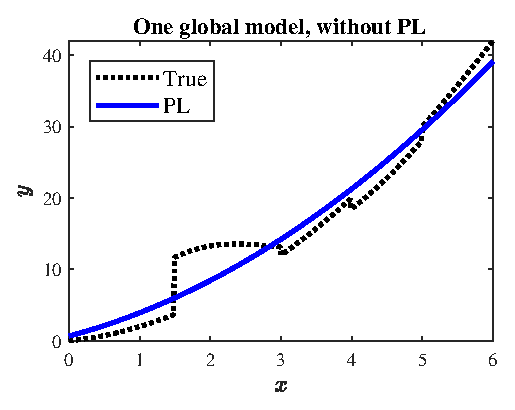
\includegraphics[width=.47\linewidth,clip]{Fig3a}}
\subfigure[]{\label{fig:gRMSE0}    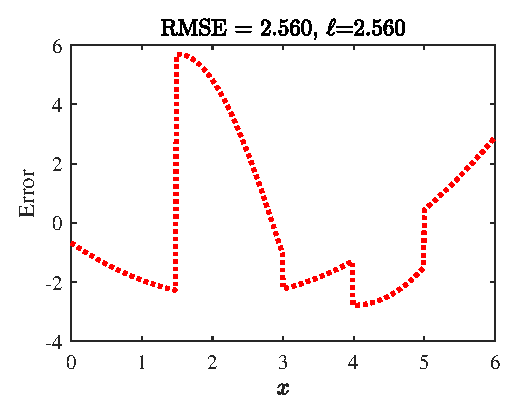
\includegraphics[width=.47\linewidth,clip]{Fig3b}}
\caption{The general idea of PL, illustrated by a simple 1D curve fitting problem. (a) fitting by one global model $f_g(x)$; (b) the fitting error of $f_g(x)$.} \label{fig:gPL}
\end{figure}

The first step is to build a global model $f_g(x)$ using all $N$ training examples. The fitted model is $f_g(x)=0.68+2.63x+0.63x^2$, plotted as the solid blue curve in Fig.~\ref{fig:gPL0}. The fitting errors are shown in Fig.~\ref{fig:gRMSE0}. Clearly, the RMSE is large, i.e., a single global model cannot fit the data well.

By visual examination of Fig.~\ref{fig:gRMSE0}, we can see that the fitting errors are large when $x\in[1.5,3]$. So, the next step is to build a patch model for $x\in[1.5,3]$. Using only the training examples within this patch, we obtain the first patch model $f_1(x)=1.65+9.81x-2.01x^2$. $f_g(x)$ and $f_1(x)$ together reduce the training RMSE from $2.560$ to $1.654$, and the loss $\ell$ from $2.560$ to $1.967$, as shown in Fig.~\ref{fig:gRMSE1}. The fitting accuracy is improved, but the RMSE may still be too large. So, a second patch model may be needed.

By visual examination of Fig.~\ref{fig:gRMSE1}, we can see that the fitting errors are large when $x\in[4,5]$. So, the next step is to build a patch model for $x\in[4,5]$. Using only the training examples within this patch, we obtain the second patch model $f_2(x)=19.29-8.03x+1.96x^2$. $f_g(x)$, $f_1(x)$ and $f_2(x)$ together further reduce the training RMSE to $1.332$, and the loss to $1.753$, as shown in Fig.~\ref{fig:gRMSE2}.

Assume at this point we do not want to add more patches. The final step is then to update the default global model, using all training examples outside of the two patches.  The updated global model is $f'_g(x)=x+x^2$, identical to the last case in (\ref{eq:g}). This step reduces the RMSE to $0.026$, and the loss to $0.035$, as shown in Fig.~\ref{fig:gRMSE3}.

For the above simple 1D curve fitting example, the final PL model can be easily represented as:
\begin{align}
y=\left\{\begin{array}{ll}
           f_1(x)=1.65+9.81x-2.01x^2, & x\in[1.5,3] \\
           f_2(x)=19.29-8.03x+1.96x^2, & x\in[4,5] \\
           f'_g(x)=x+x^2, & \mbox{otherwise}
         \end{array}\right. \label{eq:g2}
\end{align}

Generally, once the PL models are trained, the logic for determining which model to use for a new input is shown in Fig.~\ref{fig:PLmodel}. We first determine if the input falls into any patch. If yes, then the corresponding patch model is used to compute the output. Otherwise, the global model is used.

\begin{figure}[htbp]         \centering
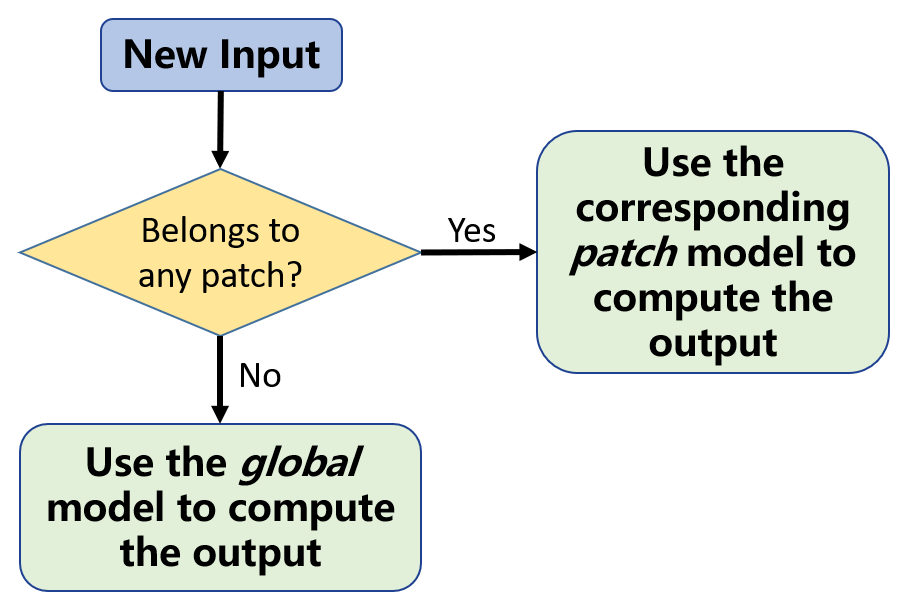
\includegraphics[width=.6\linewidth,clip]{Fig4}
\caption{The logic for determining which model to use in PL.} \label{fig:PLmodel}
\end{figure}


For a well-optimized fuzzy system, transition from one rule partition to another changes the functional form of the input-output mapping. For example,  assume $x_m$ is the only input of the TSK fuzzy system, which has the following three rules:
\begin{align*}
R_1: &\mbox{ IF } x_m \mbox{ is } A_1, \mbox{ THEN } y=y_1(x_m)\\
R_2: &\mbox{ IF } x_m \mbox{ is } A_2, \mbox{ THEN } y=y_2(x_m)\\
R_3: &\mbox{ IF } x_m \mbox{ is } A_3, \mbox{ THEN } y=y_3(x_m)
\end{align*}
where $y_1(x_m)$, $y_2(x_m)$ and $y_3(x_m)$ are different functions of $x_m$. In Partition $P(1|x_m)$, only Rule $R_1$ is fired, and hence the fuzzy system output is $y=f_1(x_m)$; in Partition $P(2|x_m)$, both Rules $R_1$ and $R_2$ are fired, and hence the fuzzy system output is:
\begin{align}
y=\frac{\mu_{A_1}(x_m)y_1(x_m)+\mu_{A_2}(x_m)y_2(x_m)}{\mu_{A_1}(x_m)+\mu_{A_2}(x_m)};
\end{align}
in Partition $P(3|x_m)$, only Rule $R_2$ is fired, and hence the fuzzy system output is $y=f_2(x_m)$. Clearly, the functional forms of $y$ in the different rule partitions are different. It is reasonable to believe this is because the (unknown) groundtruth functional form changes significantly from one rule partition to another, and hence the fuzzy system uses different functional forms in different rule partitions to accommodate it. Thus, we can consider each such partition as a patch candidate\footnote{This is just one simple way to initialize the patch candidates. There may be better ways to do this.}.

According to Pedrycz \cite{Pedrycz2018}, \emph{``by information granules one regards a collection of elements drawn together by their closeness (resemblance, proximity, functionality, etc.) articulated in terms of some useful spatial, temporal, or functional relationships. Subsequently, Granular Computing is about representing, constructing, processing, and communicating information granules."} All points within a first-order rule partition fire the same number of same rules, and hence they resemble each other. So, each first-order rule partition can be viewed as an information granule, and PL can be viewed as a form of granular computing.

\subsection{Implementation Details}

For the ease of programming implementation, we can use a single index $k\in[1,K]$ to denote a patch candidate (first-order rule partition) $(P(k_1|x_1),P(k_2|x_2),...,P(k_M|x_M))$, where
\begin{align}
k&=(k_1-1)\cdot \prod_{m=2}^M K_m+(k_2-1)\cdot \prod_{m=3}^M K_m \nonumber \\
 &\quad +\cdots+(k_{M-1}-1)\cdot K_M+k_M\nonumber \\
&=k_M+\sum_{m=1}^{M-1}\left[ (k_m-1)\cdot \prod_{p=m+1}^M K_p\right] \label{eq:k}
\end{align}
For example, assume the fuzzy system has two inputs ($M=2$), $x_1$ and $x_2$, each with five first-order rule partitions ($K_1=K_2=5$) shown in Fig.~\ref{fig:Partition}. Then, (\ref{eq:k}) becomes $k=(k_1-1)\times K_2+k_2$. The partition $(P(1|x_1),P(1|x_2))$ is mapped to $k=(1-1)\times 5+1=1$, $(P(1|x_1),P(2|x_2))$ to $k=(1-1)\times 5+2=2$, $\cdots$, $(P(2|x_1),P(1|x_2))$ to $k=(2-1)\times5+1=6$, $\cdots$, and $(P(5|x_1),P(5|x_2))$ to $k=(5-1)\times 5+5=25$.


For a given $k\in[1,K]$, we can also map it back to a first-order rule partition $(P(k_1|x_1),P(k_2|x_2),...,P(k_M|x_M))$:
\begin{align}
k_1&=int\left(\frac{k-1}{\prod_{m=2}^M K_m}\right)+1 \label{eq:k1}\\
k_2&=int\left(\frac{k-1-(k_1-1)\cdot \prod_{m=2}^M K_m}{\prod_{m=3}^M K_m}\right)+1\\
k_m&=int\left(\frac{k-1-\sum_{i=1}^{m-1}\left[(k_i-1)\cdot \prod_{p=i+1}^M K_p\right]}{\prod_{p=m+1}^M K_p}\right)+1\\
k_M&=k-\sum_{m=1}^{M-1}\left[ (k_m-1)\cdot \prod_{p=m+1}^M K_p\right] \label{eq:kM}
\end{align}
where $int(x)$ means the integer part of $x$, e.g., $int(2.0)=2$ and $int(2.9)=2$. Using again the above example, when $k=6$, we have $k_1=int(\frac{k-1}{K_2})+1=int(\frac{6-1}{5})+1=2$ and $k_2=k-(k_1-1)\times K_2=6-(2-1)\times 5=1$, and hence the mapped first-order rule partition for $k=6$ is $(P(2|x_1),P(1|x_2))$.

In summary, the pseudo-code\footnote{A sample Matlab implementation is available at https://github.com/drwuHUST/Patch-Learning.} in Algorithm~\ref{alg:PLFS} implements the three generic PL steps described at the beginning of Section~\ref{sect:PL} using fuzzy systems. Its limitations and potential improvements are discussed in Section~\ref{sect:limitations}, after some experiments to demonstrate its capability are described in the next section.

\begin{algorithm}[htbp]
\KwIn{$N$ labeled training examples, $\{(\mathbf{x}_n,y_n)\}^N_{n=1}$, where $\mathbf{x}_n\in\mathbb{R}^{M\times 1}$\;
\hspace*{9mm} $T$ unlabeled examples, $\{\mathbf{x}_t\}_{t=1}^T$\;}
\KwOut{The PL model predictions for $\{\mathbf{x}_t\}_{t=1}^T$.}
\tcp{Train the PL model}
Train a global fuzzy model using all $N$ training examples\;
\For{$m=1,...,M$}
{Identify the first-order rule partitions for the $m$th input domain of the global fuzzy model\;}
Index the partitions using $k$ in (\ref{eq:k})\;
Include all partitions in the candidate pool\;
$l=1$\;
    \While{$l\le L$}{
    Identify from the candidate pool the partition giving the maximum SSE\;
    Record the location of the partition as the $l$th patch\;
    Train a patch fuzzy model using only the training examples within the $l$th patch\;
    \If{the $l$th model is successfully trained\footnotemark{}}
    {$l=l+1$\;}
    Remove the above patch from the candidate pool\;}
\caption{PL using fuzzy systems.} \label{alg:PLFS}
\end{algorithm}



\begin{table}[h] \centering \setlength{\tabcolsep}{1.5mm}
\caption{RMSEs, APEs and losses of Bagging and LSBoost in 3D manifold fitting.}   \label{tab:E3}
\begin{tabular}{c|c|cccccc}   \hline
 & & \multicolumn{6}{c}{Number of weak learners}\\ \cline{3-8}
&  & 1 & 2 & 3 &4 &5 & 6\\ \hline
\multirow{2}{*}{Bagging}&RMSE & 0.2192 &   0.2291 &   0.1546  &  0.1924 & 0.1863 & 0.2337\\
&APE & 0.0157 &   0.0163 &   0.0111 &   0.0138 & 0.0134 & 0.0168\\ \hline
\multirow{2}{*}{LSBoost}&RMSE & 1.6534 &   1.2820 &   0.9823  &  0.8261 & 0.7361 & 0.6797\\
&APE & 0.0157 &    0.0822 &   0.0633 & 0.0562 & 0.0496 & 0.0459\\ \hline
\end{tabular}
\end{table}



\section{Conclusions} \label{sect:conclusion}

When the performance of a machine learning model is not satisfactory, there are different strategies to improve it, including designing a deeper, wider, and/or more nonlinear model, and ensemble learning (aggregate multiple base/weak learners in parallel or in series). This paper has proposed a novel strategy, \emph{patch learning}, to improve the performance of a machine learning model. It first identifies a few patches from the initial model, which contribute the most to the learning error. Then, a (local) patch model is trained for each such patch, using only training examples falling into the patch. Finally, a global model is trained using training data that do not fall into any patch. To use the PL model, we first determine if the input falls into any patch. If yes, then the corresponding patch model is used to compute its output. Otherwise, the global model is used. Five experiments on different regression problems verified the effectiveness of the proposed PL approach: as more patch models are added, the overall RMSE decreases. We also defined a loss function for determining the optimal number of patches, considering the trade-off between RMSE and model complexity.

It should be emphasized that although this paper focuses on PL using fuzzy systems, the idea is generic: any machine learning algorithm can be used as the patch model, and the patch models can also be trained using different machine learning algorithms.


\section*{Acknowledgement}
This research was supported by the National Natural Science Foundation of China Grant 61873321.



\bibliographystyle{IEEEtran}\bibliography{drwubib}


\begin{IEEEbiography}[{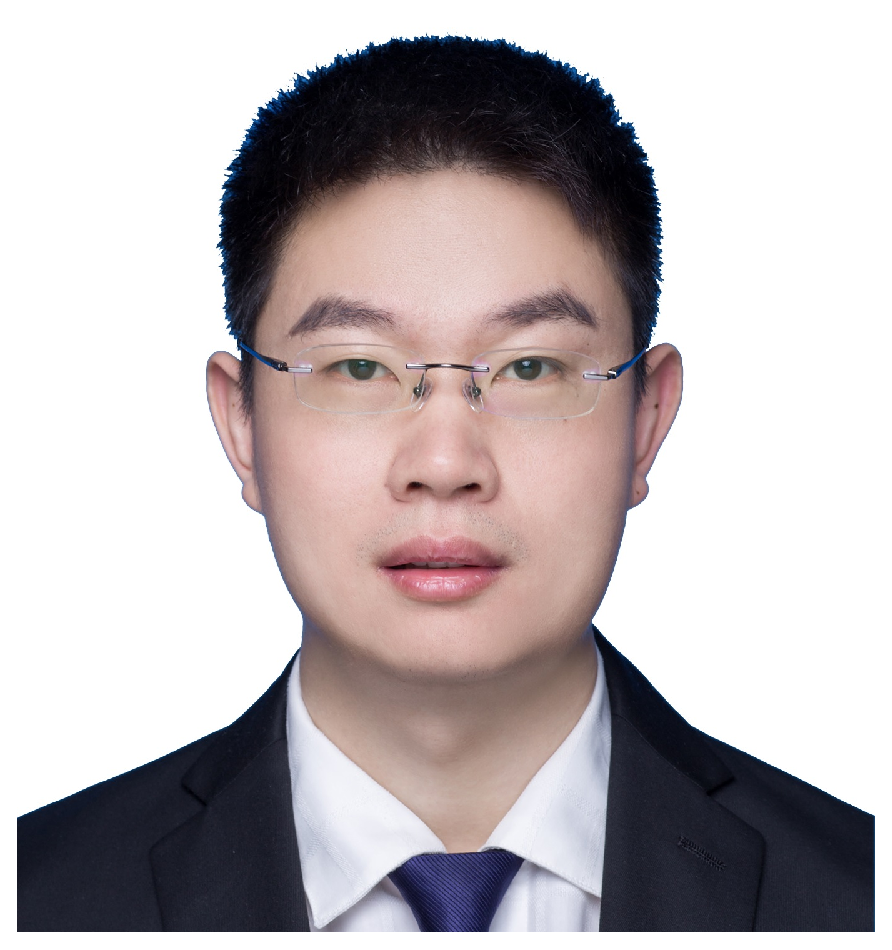
\includegraphics[height=1in,clip,keepaspectratio]{Wu}}]{Dongrui~Wu} (S'05-M'09-SM'14) received the BE degree in automatic control from the University of Science and Technology of China in 2003, the ME degree in electrical engineering from the National University of Singapore in 2005, and the PhD degree in electrical engineering from the University of Southern California in 2009. He is now Professor in the School of Artificial Intelligence and Automation, Huazhong University of Science and Technology, Wuhan, China, and Deputy Director of the Key Laboratory of Image Processing and Intelligent Control, Ministry of Education. His research interests include affective computing, brain-computer interface, computational intelligence, and machine learning. He has more than 110 publications, including a book entitled \emph{Perceptual Computing} (Wiley-IEEE Press, 2010).

Prof. Wu received the IEEE Computational Intelligence Society Outstanding PhD Dissertation Award in 2012, the IEEE TRANSACTIONS ON FUZZY SYSTEMS Outstanding Paper Award in 2014, the NAFIPS Early Career Award in 2014, the IEEE Systems, Man and Cybernetics (SMC) Society Early Career Award in 2017, and the IEEE SMC Society Best Associate Editor Award in 2018. He was also a finalist of another three Best Paper Awards. He was/is an Associate Editor of the IEEE TRANSACTIONS ON FUZZY SYSTEMS (2011-2018), the IEEE TRANSACTIONS ON HUMAN-MACHINE SYSTEMS (2014-), the IEEE COMPUTATIONAL INTELLIGENCE MAGAZINE (2017-), and the IEEE TRANSACTIONS ON NEURAL SYSTEMS AND REHABILITATION ENGINEERING (2019-).
\end{IEEEbiography}

\begin{IEEEbiography}[{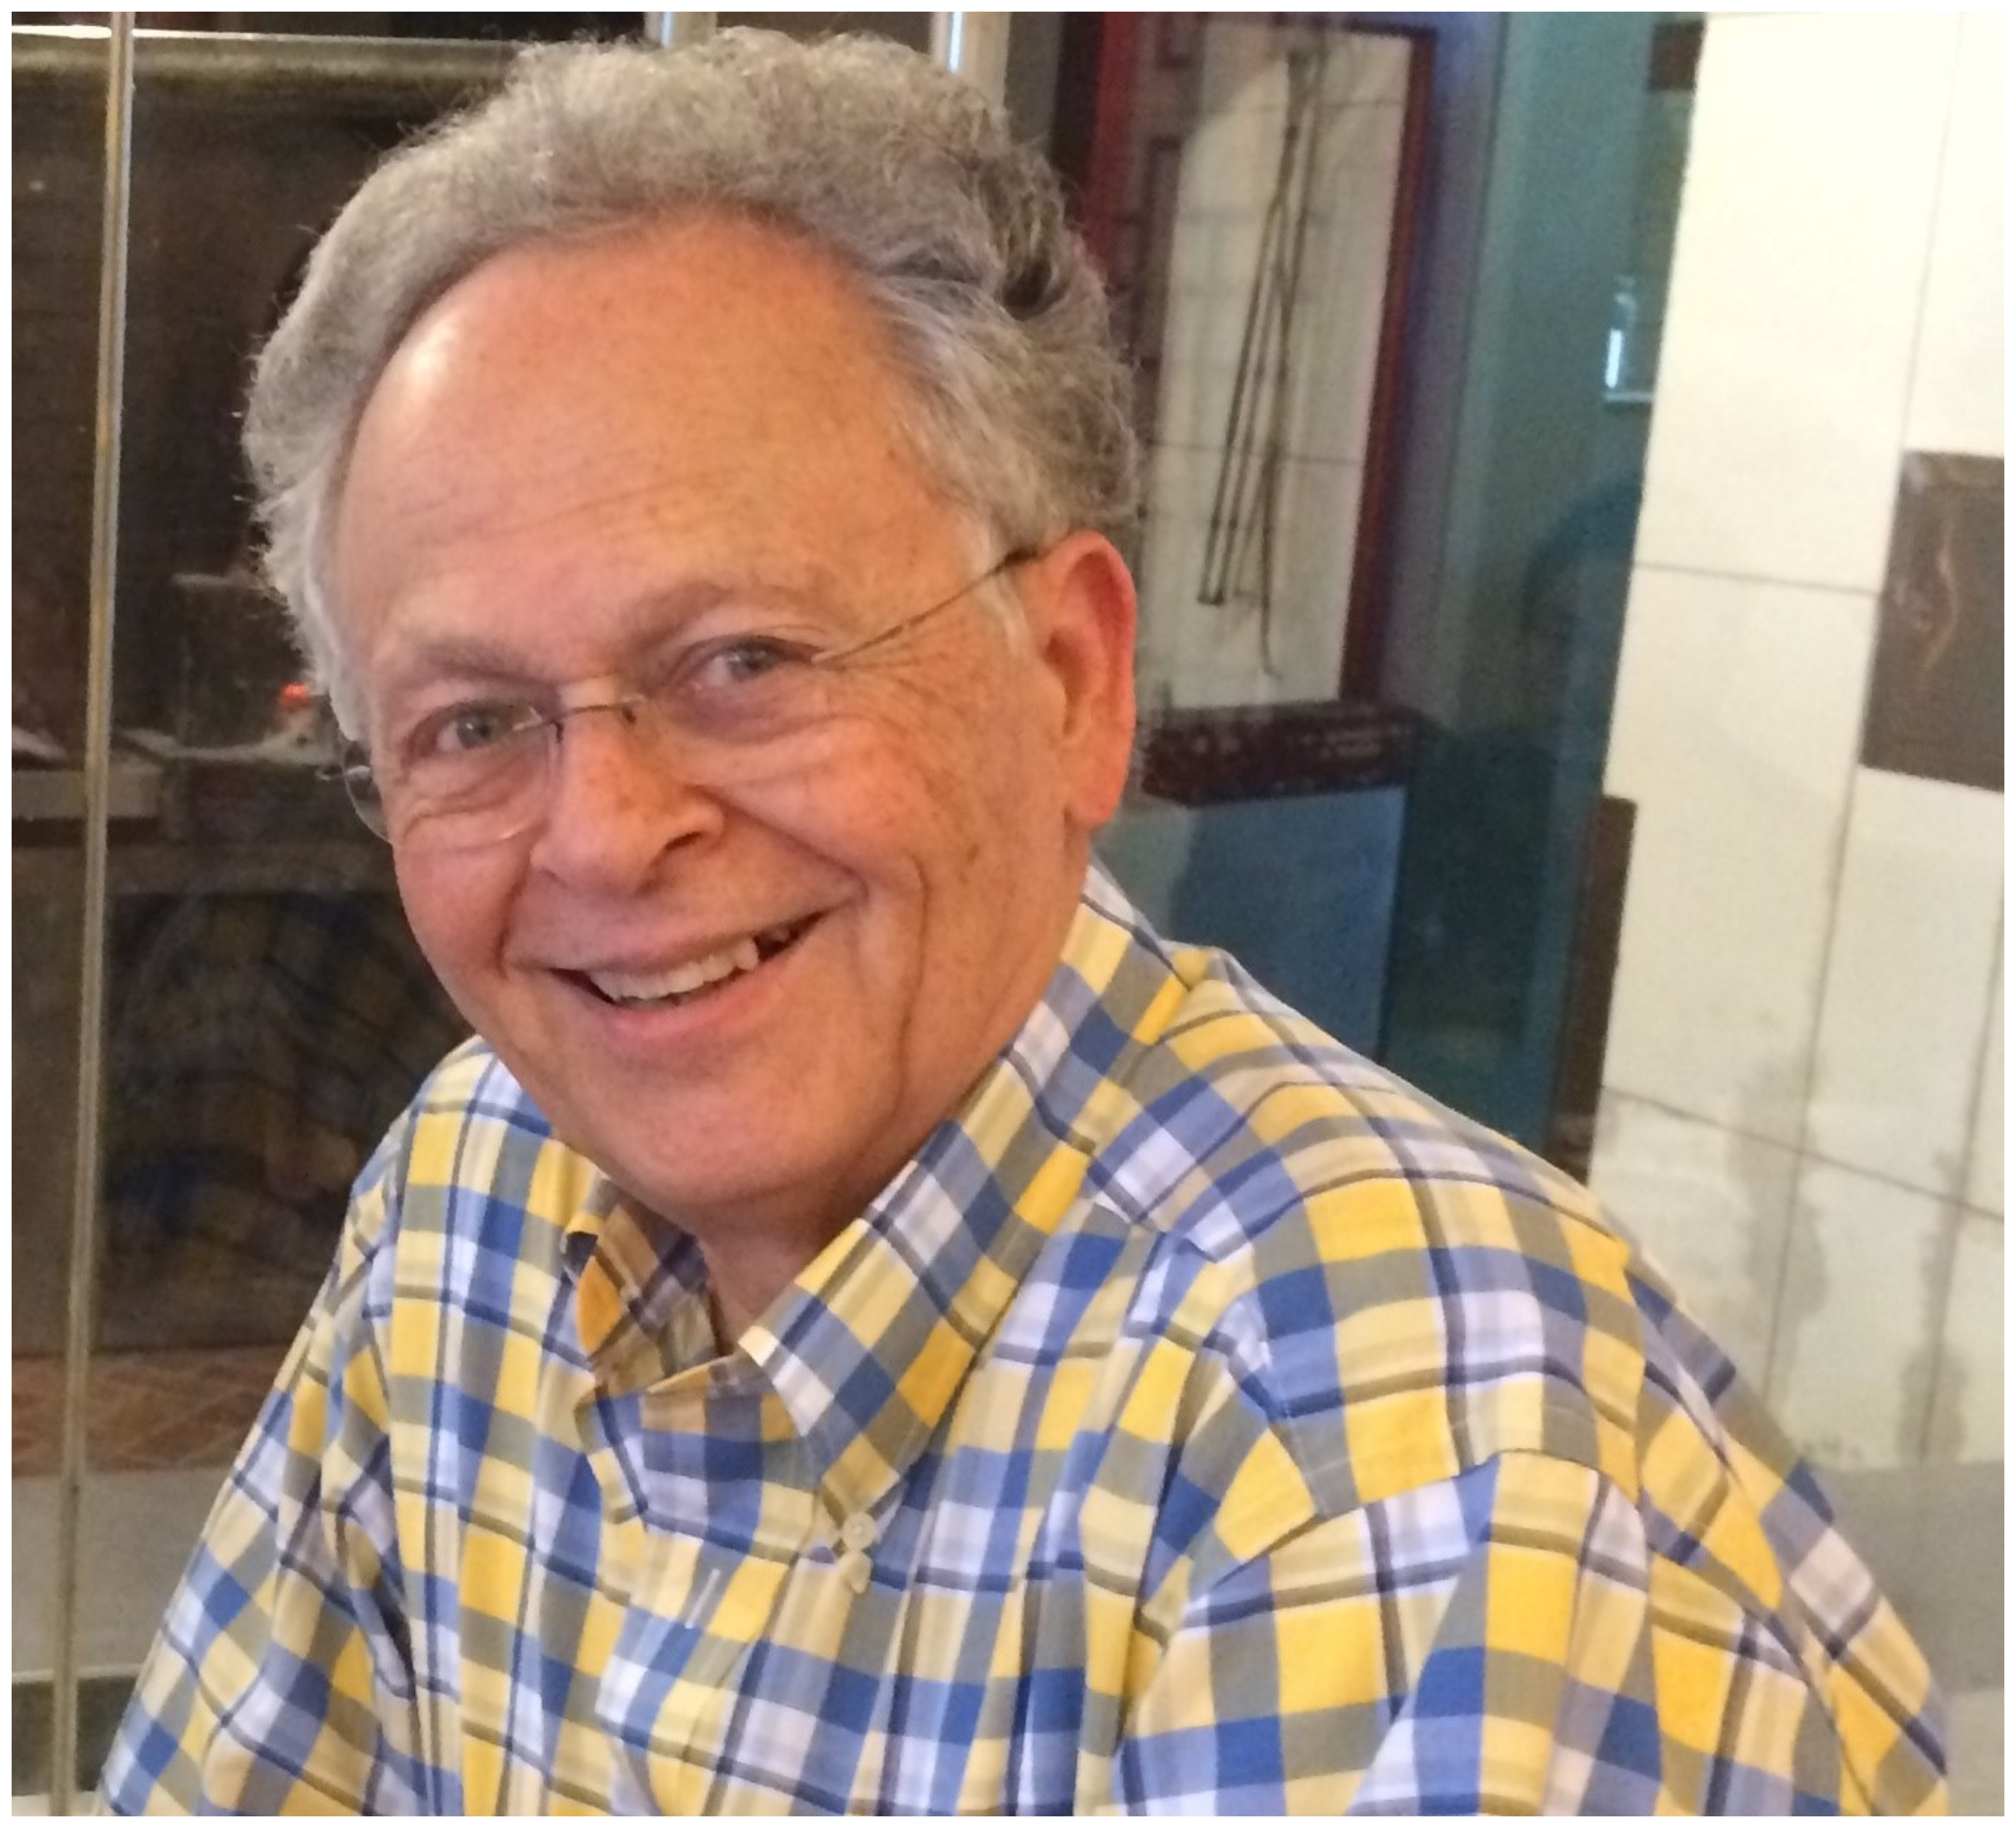
\includegraphics[width=1in,clip,keepaspectratio]{Mendel}}]{Jerry M. Mendel} (LF'04) received the Ph.D. degree in electrical engineering from the Polytechnic Institute of Brooklyn, Brooklyn, NY, in 1963. Currently, he is Emeritus Professor of Electrical Engineering at the University of Southern California in Los Angeles,  where he has been since 1974. He is also Tianjin 1000-Talents Foreign Experts Plan Endowment Professor and Honorary Dean of the College of Artificial Intelligence, Tianjin Normal University, Tianjin, China.

He has published over 570 technical papers and is author and/or co-author of 13 books, including Uncertain Rule-based Fuzzy Systems: Introduction and New Directions, 2nd ed. (Springer 2017), Perceptual Computing: Aiding People in Making Subjective Judgments (Wiley \& IEEE Press, 2010), and Introduction to Type-2 Fuzzy Logic Control: Theory and Application (Wiley \& IEEE Press, 2014). He is a Life Fellow of the IEEE, a Distinguished Member of the IEEE Control Systems Society, and a Fellow of the International Fuzzy Systems Association. He was President of the IEEE Control Systems Society in 1986, a member of the Administrative Committee of the IEEE Computational Intelligence Society for nine years, and Chairman of its Fuzzy Systems Technical Committee and the Computing With Words Task Force of that TC. Among his awards are the 1983 Best Transactions Paper Award of the IEEE Geoscience and Remote Sensing Society, the 1992 Signal Processing Society Paper Award, the 2002 and 2014 Transactions on Fuzzy Systems Outstanding Paper Awards, a 1984 IEEE Centennial Medal, an IEEE Third Millenium Medal, a Fuzzy Systems Pioneer Award (2008) from the IEEE Computational Intelligence Society for ``fundamental theoretical contributions and seminal results in fuzzy systems"; and, 2015 USC Viterbi School of Engineering Senior Research Award. His present research interests include: type-2 fuzzy logic systems and computing with words.
\end{IEEEbiography}

\end{document}
